\chapter{Introducció als models}

En els capítols següents es dissenya un model matemàtic per a la
gestió en bases de dades de la multiresolució de sèries temporals.  Es
defineixen els objectes que ens permeten modelar l'estructura de les
dades i els operadors que s'hi poden aplicar.

La definició del model s'estructura en dos capítols:

\begin{itemize}
\item Un model pels \gls{SGST}  que defineix mesura i sèrie temporals.
\item Un model pels \gls{SGSTM} que defineix buffer, disc, subsèrie
  resolució, sèrie temporal multiresolució i esquema de
  multiresolució. Aquest model es defineix a partir del model de \gls{SGST}.
\end{itemize}



  
En aquest capítol d'introducció, resumim els objectius de la definició
dels models i aclarim alguns termes i conceptes que altrament podrien
resultar confusos.  Primer, relacionem el concepte de model matemàtic
pels \gls{SGBD} de \textref{sec:art:sgbd} amb el model que
proposem. Segon, introduïm el context i els supòsits que utilitzarem a
l'hora de treballar amb les sèries temporals en els conceptes de
\textref{sec:art:seriestemporals}.  Tercer, introduïm les
característiques principals de la multiresolució i la motivació per a
definir-la.


\section{Introducció als conceptes de model}

%Sobre què és una base de dades i un sistema que la gestiona
\paragraph{Què és una base de dades i un sistema que la gestiona.}
Una definició més particular de base de dades que l'exposada en
la~\autoref{sec:art:sgbd} és ``conjunt de dades organitzades segons
una estructura coherent i accessibles des de més d'un programa o
aplicació, de manera que qualsevol d'aquestes dades pot ésser extreta
del conjunt i actualitzada, sense que això afecti ni l'estructura del
conjunt ni les altres dades'' \parencite[s.~v.~base de dades]{termcat}
amb la corresponent definició per als sistemes que les gestionen de
``sistema informàtic que permet la gestió automàtica d'una base de
dades, generalment la creació, l'emmagatzematge, la modificació i la
protecció de les dades que s'hi contenen'' \parencite[s.~v.~sistema de
gestió de bases de dades]{termcat}.  En aquest cas, hem de precisar
que en els capítols següents ens centrem en la teoria dels sistemes
d'informació, basant-nos en el model
relacional \parencite{date04:introduction8}, per a proposar el model
lògic i deixem de banda els aspectes més d'implementació informàtica,
com per exemple accedir o manipular físicament les dades.

D'aquestes definicions cal destacar la precisió en els termes
d'estructura, organitzada i coherent, és a dir que s'enumeren els
requisits per al correcte emmagatzematge de les dades en concordança
amb l'expressat en el model relacional.  En aquestes definicions, a
més, caldria afegir que els \gls{SGBD} han de ser capaços d'inferir
informació, és a dir a partir de les dades emmagatzemades deduir-ne de
noves mitjançant les consultes.





%Sobre model aproximat i model exacte
\paragraph{Què es modelitza amb exactitud i què amb aproximació.}
Els models de \gls{SGST} i \gls{SGSTM} que proposem són models lògics
matemàtics, és a dir són models formals i abstractes que defineixen
amb exactitud l'estructura i la manipulació d'unes dades
independentment de la realitat.  Així doncs es defineixen models de
\gls{SGBD} i es presenten com un model matemàtic formal, per tant la
realitat que es modelitza són els \gls{SGBD}. Un cop definit el model,
aleshores els \gls{SGBD} s'usen com a eines simbòliques per a
modelitzar la realitat, és a dir en el procés de dissenyar un model
que aproximi i simplifiqui una realitat. Cal no confondre la definició
del model formal matemàtic amb la interpretació del model en una
realitat concreta.

Tot i tenir tot el sentit matemàtic, un model lògic abstracte no té
sentit pràctic si no es té en compte la descripció que fa de la
realitat, és a dir que també s'ha d'interpretar el significat que té
el model en la realitat.  Aquest procés d'interpretació construeix un
model aproximat i simplificat de la realitat; és a dir que consisteix
en definir per a un determinat context quines variables hi ha, de quin
tipus són els valors, quina forma tenen, com s'interpreten, etc.  Els
\gls{SGBD} descriuen la realitat mitjançant predicats que indiquen
quins fets es consideren certs, però els models de \gls{SGBD}
parteixen d'assumir que aquests predicats són la realitat, en tot cas
deixen per altres teories l'avaluació de com els predicats s'aproximen
a la realitat i deixen per als usuaris la interpretació del significat
dels predicats a la realitat llevat d'allò que es pot expressar
mitjançant regles d'integritat.


En l'àmbit dels \gls{SGST}, el model descriu
exactament com a fet cert la mesura d'un valor i deixen que altres
teories, com per exemple podria ser la teoria de la mesura, avaluïn
fins a quin punt el valor mesurat s'aproxima a la
realitat. Particularment, si els fets descriuen allò que s'ha mesurat
aleshores podem plantejar el cas de mesurar valors desconeguts, mentre
si descriuen directament allò que realment val la variable en el model
no hi tenen cabuda les propietats de l'adquisició de la mesura. 
En l'àmbit dels \gls{SGSTM}, el model descriu com a fet cert unes
resolucions de la sèrie temporal i mitjançant altres teories, com per
exemple la teoria de la informació, s'avalua com s'aproximen a la
informació d'una sèrie temporal original.



%  D'alguna manera, els SGBD descriuen exactament els
% fets que es coneixen i mitjançant altres teories es dedueix en quina
% mesura aquests fets coneguts s'aproximen a la realitat (particularment
% un fet descrit com a cert en un SGBD pot ser totalment esbiaixat de la
% realitat però això no se n'ocupen els SGBD; és a dir el predicat exacte és el d'allò que és observat tot i que mitjançant altres teories es pot assegurar un predicat d'allò que és la realitat).
% ; i per tant
% la interpretació del significat dels models matemàtics a la realitat,
% i com a conseqüència la modelització aproximada de la realitat, depèn del
% conjunt del model lògic de SGBD més altres teories. 


% Kopetz en el llibre de temps real (capítol 2 o 3?) diu que un model té l'objectiu d'estudiar una realitat simplificada per a facilitar la comprensió d'una determinada característica. Potser la definició que fa i la intencionalitat que té no és ben bé la mateixa que el tipus de model que parlem aquí? Si és el cas potser estaria bé fer notar que hi ha diferències en el concepte de model segon l'àmbit i que aquí s'utilitza en tal sentit.

% Per exemple, Fabian Pascal parla de representar la realitat de manera simple (i no tant de simplificar la realitat):
% ``For the informational purpose that RM satisfies--inferencing facts that are logical implications of facts represented in databases--the RM is superior, because it is the simplest way to guarantee logically correct results with respect to the real world and it has the highest scope-to-simplicity ratio: it can represent any reality with the least and simplest of constructs''




\paragraph{Quin nivell es modela.}
En la~\autoref{sec:art:sgbd} s'han nombrat els tres nivells de
l'arquitectura dels \gls {SGBD}: el físic, el lògic i el d'usuari.
Els models que es proposen pertanyen al nivell lògic, és a dir són
models lògics per les dades i pel comportament dels \gls{SGST} i
\gls{SGSTM}.  En \textref{sec:implementacio:python} es
proposen implementacions per a aquests models i per tant pertanyen al
nivell físic.  En alguns exemples i descripcions de propietats dels
models, s'avalua el significat en un context particular del model, és
a dir la semàntica del model, cosa que pertany a descriure com els
usuaris poden interpretar el model lògic per a modelitzar la realitat.
% és a dir descriu la relació entre el nivell lògic i el d'usuari \todo{???}





\paragraph{Àlgebra o càlcul relacional.} Els models que definim són
similars a l'àlgebra relacional. L'àlgebra relacional es basa en la
teoria de conjunts, que és més propera a la definició d'una sèrie
temporal com a conjunt de mesures i a aplicar-hi operacions de manera
prescriptiva. Alternativament, el càlcul relacional, que com s'ha
descrit a la~\autoref{sec:art:sgbd} és equivalent a
l'àlgebra relacional, es basa en la lògica de predicats i és més
proper a aplicar les operacions de manera descriptiva. Això no
obstant, en les definicions usem tant l'àlgebra com la lògica de
conjunts segons convingui i faciliti la comprensió de les definicions.




% \paragraph{Model com a relació o com a tipus de dades.} 
% Aquesta és una pregunta complicada. Sobretot perquè el model
% relacional no ho aclareix; descriu les relacions com si no fossin un
% tipus de dades tot i que després accepta que hi hagi relacions amb
% atributs de relacions. Nosaltres volem presentar un model de gestió
% de dades per a tipus complexos, les sèries temporals i les
% multiresolució, i aleshores veiem la necessitat d'abordar-ho des del
% model relacional al complet (com si fossin uns SGBD específics per a
% aquelles tasques). Ara bé, en un SGBD genèric aquests models de
% dades s'entendrien com a tipus de dades.







\section{Introducció a les sèries temporals}


Una sèrie temporal és una representació per a unes variables o
magnituds físiques que evolucionen al llarg del temps.  En els models
usarem les sèries temporals des de la visió més genèrica possible, és
a dir una sèrie temporal com a conjunt de dades que s'han adquirit en
uns certs instants de temps.  En aquest sentit, les sèries temporals
poden representar dades molt variades i que pertanyen a àmbits molt
diferents.


Les mateixes dades, la variació en el temps de magnituds, són
estudiades en altres teories com per exemple la teoria del senyal; de
fet les sèries temporals són una de les eines en aquesta teoria.  Això
no obstant, en les anàlisis aquests senyals normalment s'assumeixen
com a periòdics, afitats en freqüència, valors adquirits com a
seqüències equiespaiades i amb una forta anàlisi en els components
freqüencials. %
L'aproximació que presentem en sèries temporals és un raonament
similar més genèric però més propi de l'àlgebra discreta matemàtica
mentre que la teoria del senyal és més pròpia de l'àmbit del càlcul
matemàtic. És a dir, que les sèries temporals tindran una forma més
genèrica on per exemple es podrà tenir en compte la posició absoluta
en el temps de les mostres o es podrà tolerar l'inframostreig.  Això
no treu, però, que quan una sèrie temporal compleix amb els paràmetres
de senyal digital, les operacions més adients a aplicar-hi siguin les
del processament digital del senyal.

%5El teorema de mostreig de Shanon-Nyquist és vital en els senyals digitals?
% Un senyal digital és un senyal (una quantitat que té informació) representat per una seqüència de valors discrets de la quantitat. Un senyal analògic és un senyal representat per una quantitat que varia contínuament.



Així doncs, l'estudi genèric proposat de les sèries temporals no
pretén substituir aquests estudis propis de cada àmbit sinó que pretén
oferir una visió més àmplia i comuna a totes aquestes dades i oferir
un estudi per a aquelles dades que no tenen un comportament clarament
definit. Aquest és el cas, per exemple, de les dades adquirides en un
monitoratge en entorns no controlats d'una variable física: aquestes
variables són aleatòries, el temps d'adquisició pot ser irregular i
per tant cal estudiar-les com a sèries temporals genèriques.
Cal dir, que a vegades les sèries temporals es redueixen a seqüències
temporals, és a dir a estudis de dades on només importa l'ordre en què
s'han adquirit i el període d'adquisició es constant. No fem
aquesta reducció sinó que tractem les sèries temporals des del punt de
vista més genèric on cal saber també la posició de temps absoluta que
ocupen i la distància de temps entre els valors.
Aquests estudis més particulars de les sèries temporals, els quals es
focalitzen i simplifiquen algunes propietats, permeten concentrar-se
més en àmbits específics i oferir solucions molt ben raonades.  Per
tant és interessant poder incorporar aquests estudis en els models, en
aquest sentit per exemple utilitzarem conceptes de la teoria del
senyal per a interpretar propietats de les sèries temporals.




\paragraph{Interpretació de la sèrie temporal.} 
La interpretació genèrica d'una sèrie temporal és un conjunt de
predicats `en el temps $t$ la variable observada té el valor $v$'
pertanyents a una mateixa variable o fenomen físic.  De forma més
particular, i en una interpretació més lligada a l'adquisició i
monitoratge continu de fenòmens, una sèrie temporal indica la mesura
d'un valor en un temps, és a dir que el fet que es constata com a cert
és que segons un rellotge i un aparell de mesura s'ha adquirit una
parella de temps i valor.  


El models de \gls{SGBD} defineixen la metodologia i asseguren la
correctesa en la inferència d'informació a partir dels fets que es
donen com a certs. Des del punt de vista del model relacional, alhora
es donen com a falsos els fets que no són constatats; és a dir que si
en una sèrie temporal hi apareix una mesura en un temps $t$ de valor
$v$ significa alhora que és fals que en aquell instant s'ha mesurat un
altre valor diferent de $v$. Particularment, en el cas que en una
sèrie temporal no hi apareix un temps $t$ significa que és fals que en
aquell instant s'ha mesurat qualsevol valor; així, si s'ha mesurat
però s'ha obtingut un valor erroni aleshores hauria d'aparèixer marcat
amb un valor especial.

Atesa aquesta interpretació de valor adquirit en un instant de
temps per a una mateixa variable observada, en una sèrie temporal no
hi pot haver instants de temps repetits. Altrament, no tindria sentit
que un mateix aparell hagués mesurat alhora dos valors diferents en el
mateix instant.
  


% En alguns casos la interpretació, a més, es pot particularitzar,
% com en els casos descrits de senyal i so. O al revés, unes dades
% que es consideraven un senyal de so es tracten genèricament com a
% sèries temporals.

% Particularment, en els casos similars a la consulta de les mitjanes
% mensuals de temperatures i a les particularitzacions amb seqüències,
% el temps és discret i no fa tanta referència a un posicionament
% absolut sobre la línia temporal.



%\paragraph{Modelització de la realitat amb sèries temporals.} %?
\paragraph{Semàntica de les sèries temporals.}
Les sèries temporals s'utilitzen per a modelitzar aspectes de la
realitat i per tant per a cada cas cal estudiar-ne l'adequació. Aquest
no és l'objectiu central dels models que presentem, tot i que cal
plantejar alguns aspectes semàntics per a poder comprendre'n la
utilitat. Així, cal tenir en compte dues consideracions.


Per una banda, en el context del monitoratge, per a estudiar la
deducció d'informació sobre la variable mesurada a partir del procés
d'adquisició s'ha de complementar amb les teories adients.  Per
exemple si l'aparell de mesura està avariat la informació inferida en
el \gls{SGST} serà certa des del punt de vista que aquell és el valor
mesurat per l'aparell però, evidentment, no serà cert que la variable
hagi tingut aquell valor. De fet, aquest és el principi d'inferència
d'informació que segueix el model relacional de bases de dades: a
partir dels fet que es donen com a certs estableixen com a certa la
informació que s'infereix, els models asseguren que aquest raonament
sigui correcte, però responsabilitzen a l'usuari d'interpretar si
aquella operació efectivament es correspon amb la informació que vol
inferir. És a dir, els operadors només tenen en compte l'estructura de
les dades i el significat i dels operadors en un context és extern al
model; com de fet és el cas d'altres àlgebres que no defineixen com
s'han d'interpretar la validesa dels resultats.

%per exemple pensem en el cas de la suma on
%  la definició matemàtica no explica com s'ha d''interpretar la
%  validesa del resultat)

Per altra banda, no totes les sèries temporals són adquirides
directament, car poden ser resultat d'operacions amb altres sèries
temporals o resultat de consultes on el temps sigui una variable, com
per exemple consultar les mitjanes mensuals de temperatures. %
 %(p.ex també l'evolució al llarg del temps de la  quantitat de visites a un portal segons el país d'origen)
En aquests casos també és important no perdre de vista la
interpretació de la validesa dels resultats.




Així doncs, en els models no incloem l'etapa d'adquisició ni de
mostreig de les sèries temporals sinó que partim del fet que les
mesures ja han estat capturades i s'ha raonat sobre l'adequació
d'aquest procés. Això no obstant, cal notar que alguns \gls{SGST}
proposen el fet d'influir sobre el procés d'adquisició a partir de la
informació gestionada \parencite{madden05}, per exemple per poder
so\l.licitar d'obtenir més mostres si s'observen variacions estranyes
o per reduir la freqüència de mostreig si es considera que el sistema
té un estat estable.






En resum, les sèries temporals tenen un atribut, l'instant de temps,
que ofereix unes particularitats a l'estructura i amb què cal operar
coherentment. Tant els instants de temps com els valors poden ser de
qualsevol tipus, tot i així sobretot els exemplificarem amb nombres
reals per tal de facilitar-ne la comprensió i per ser més propers a
l'anàlisi de sèries temporals que sol focalitzar-se en mètodes
estadístics per a variables numèriques \parencite{last04:book}.


% * El temps és un nom donat al camp, qualsevol objecte que tingui la mateixa interfície que el temps pot funcionar. En el cas del valor pot ser qualsevol objecte, s'exemplifica amb reals per facilitar-ne la comprensió i per ser el més proper al time series analysis: statistical methods focused on sequences of values representing a single numeric variable [llibre-last].






\section{Introducció a la multiresolució}

La multiresolució és una tècnica que s'aplica a una sèrie temporal
per tal de compactar-ne i resumir-ne certa informació.  Bàsicament la
multiresolució consisteix a calcular un conjunt de resolucions d'una
sèrie temporal on cada resolució consisteix en aplicar una funció
d'agregació a les mesures cada cert període de temps. A més, cada
resolució inclou un paràmetre per tal d'afitar el nombre de valors
emmagatzemats.  

La idea bàsica és utilitzar la multiresolució per a descriure sèries
temporals de forma que hi hagi més resolució per a les dades més
recents i menys resolució per a les dades més antigues. Tot i així, es
podrien establir variacions d'aquesta estructura mitjançant les quals,
per exemple, es pogués retenir una resolució per a un període temporal
que ha resultat interessant o que calgués investigar més profundament.
Aquesta idea de multiresolució prové de l'\gls{SGBD}
RRDtool \parencite{rrdtool}, del qual en estudis anteriors n'hem
analitzat profundament els conceptes i n'hem abstret i formalitzat les
característiques essencials \parencite{llusa11:tfm,llusa12:ptd}.  Els
objectius principals són la formalització d'un model abstracte de
\gls{SGBD} per a la multiresolució i la inclusió de conceptes més
genèrics per tal de descriure els \gls{SGSTM} contextualitzats en els
\gls{SGST}.

En el mateix sentit que hem comparat les sèries temporals i els
senyals digitals, en altres àmbits també s'utilitzen tècniques amb
propòsits semblants als de la multiresolució.  Per exemple en el
processament del senyal digital s'utilitzen anàlisis temps-freqüència
mitjançant Fourier o \emph{wavelets} per tal d'identificar atributs en
els senyals. També com en el cas per les sèries temporals, aquestes
anàlisis del senyal tenen un fort component freqüencial i en canvi
proposem la multiresolció des d'un punt de vista més genèric.  Això no
treu, però, que fóra interessant estudiar en els \gls{SGSTM}
agregacions en el domini freqüencial.


% També hi ha l'anàlisi de les sèries temporals amb wavelet analysis. Aquest es basa en anàlisis de la freqüència dels senyals. 
% A multiresolution analysis (MRA) or multiscale approximation (MSA) is the design method of most of the practically relevant discrete wavelet transforms (DWT) and the justification for the algorithm of the fast wavelet transform (FWT). It was introduced in this context in 1988/89 by Stephane Mallat and Yves Meyer and has predecessors in the microlocal analysis in the theory of differential equations (the ironing method) and the pyramid methods of image processing as introduced in 1981/83 by Peter J. Burt, Edward H. Adelson and James Crowley.



La multiresolució aplicada a una sèrie temporal implica una selecció
d'informació i per tant és alhora una compressió de dades amb
pèrdua. Abans d'aplicar la multiresolució cal decidir quins atributs
se seleccionaran mitjançant uns paràmetres, els quals bàsicament són les
definicions del períodes de temps, les funcions que han d'agregar els atributs
i el nombre màxim de valors que s'han d'emmagatzemar.  Així doncs,
aplicar la multiresolució ha de ser una decisió consensuada, s'ha de
tenir en compte que és una compressió amb pèrdua i s'ha de pensar
adequadament la configuració dels paràmetres. O, dit d'una altra
manera, l'usuari ha de ser conscient que vol gestionar les sèries
temporals amb multiresolució; en certa manera un sistema no pot
decidir autònomament d'utilitzar la multiresolució com a equivalent a
la sèrie temporal original sense avisar l'usuari.
%
Com en els \gls{SGST}, en el cas dels \gls{SGSTM} l'usuari també ha
d'interpretar la validesa dels resultats. En aquest cas, però, la
multiresolució produeix l'efecte de compressió amb pèrdua que
estudiarem amb més detall en
\textref{sec:multiresolucio:teoriainformacio}.



El model que presentem d'\gls{SGSTM} defineix els termes i conceptes
de la multiresolució i els operadors genèrics que hi treballen. En els
capítols posteriors al model d'\gls{SGSTM}, comentarem aplicacions i variacions interessants dels \gls{SGSTM}.






\subsubsection{Característiques de la multiresolució}




\todo{revisar}


Un \gls{SGSTM} és un \gls{SGST} amb capacitats de multiresolució.  A
continuació resumim les característiques que els \gls{SGSTM} milloren
respecte als \gls{SGST}.

\begin{itemize}

\item Gran volum de dades. Els sistemes de monitoratge adquireixen una
  gran quantitat de dades dels sensors. Aquestes dades contenen
  informació que ha de ser observada, tant en línia amb l'adquisició
  com en diferit, i per tal de poder processar-la cal reduir el volum
  de dades. Una de les característiques de la multiresolució és la
  selecció i l'emmagatzematge dels segments més interessants de les
  dades. Aquests segments són el conjunt de resolucions per a cada
  sèrie temporal que l'usuari pot configurar com extreure i resumir
  mitjançant diversos períodes de temps i funcions.

\item Visualització. La multiresolució també és útil quan es
  visualitzen gràficament les sèries temporals ja que permet a
  l'usuari seleccionar el millor rang temporal i la resolució que
  s'adeqüen a la pantalla. No cal processar amb més quantitat de dades que
  la que realment es pot mostrar.


\item Validació de dades. Els sistemes de monitoratge adquireixen
  dades però poden ocórrer alguns problemes que tenen efecte en el
  procés posterior d'anàlisi de les sèries temporals. Un dels
  principals problemes ocorre quan els monitors no poden adquirir una
  dada, cosa que es coneix com a forats, o bé quan adquireixen una
  dada erròniament, com per exemple les dades atípiques o
  aberrants \parencite{quevedo10}.  Les funcions d'agregació
  d'atributs de la multiresolució poden cooperar en la validació, el
  filtratge i la reconstrucció d'aquestes dades desconegudes per tal
  de conservar històrics consistents.

\item Regularització dels instants de temps. Un altre efecte secundari
  del monitoratge ocorre quan el període de mostreig no és constant,
  és a dir quan les dades resultants no estant equiespaiades en el
  temps. Aquestes no regularitats poden provenir de fluctuacions en el rellotge de mostrejos periòdics o bé de mostrejos no periòdics basats en esdeveniments 
  \parencite{kopetz11:realtime}. Un dels objectius de la
  multiresolució és regularitzar els intervals de temps de la sèrie
  temporal, és a dir que les resolucions que en resulten són regulars
  en el temps. Aquest procés de regularització és útil per a aplicar
  posteriorment algoritmes d'anàlisi de sèries temporals que
  assumeixen que les sèries temporals són regulars, però també per a
  calcular altres resolucions de la sèrie temporal com per exemple
  observar dades periòdiques amb intervals de mes o d'any.


\item Resum de la informació. 



\todo{}

\item Information summaries. Time series analysis typically focuses on
  reconstructing the original signal. However, the user objective in a
  database system is to consult some information. The multiresolution
  approach allows a lossy compression storage solution for data. Therefore
  it can be regarded as to extracting the interesting information and
  then storing it. The selected information must be determined a
  priori assuming the context where the future queries will be done.
\end{itemize}


However sometimes it may also be useful to complement \acro{MTSMS}
with other \acro{DBMS}. Not only to store the original values as a
long-term deposit consulted offline, but also to store related
information to time series such as units of values, sensor
localisation, classification tags, last measured value, etc.
Les sèries temmporals tenen una metainformació que cal guardar en una base de dades relacional (localització, etiquetes de classificació, últim valor mesurat, unitats, etc.) [dreyer]




A TSMS is a special purpose DBMS aimed at storing and managing time
series and MTSMS is a TSMS with multiresolution capabilities. Next we
describe the main requirements that a TSMS must achieve, specifically
remarking the improvements where the MTSMS can contribute.





* Aggregates, una sèrie temporal pot estar mostrant diferent informació. ex: mitjana, màxim, valor al final del període, ...






* Representació: Entre dos punts de mesura, quin valor pren la sèrie temporal?.


* Disseny del model de TSMS, aleshores veurem si una TSMS pot ser implementada com a camp d'una altra DBMS o si els DBMS no són capaços de manipular TS adequadament i cal implementar TSMS específics.

* Xarxa de sensors, tsms distribuïda. Sensor dades recents, màquina grossa històrics. Quan es llança una consulta, es llança distribuïdament: si es té prou resolució es respon sinó s'envia la consulta al sensor. [bonnet01?]

* S'ha de poder calcular incrementalment, citar data streams

* Necessitem les fórmules (els interpoladors) a trossos, en el domini dels conjunts?: sí perquè la fórmula contínua necessita mètodes númerics per calcular-se? per exemple calcular l'àrea de S(t): amb integral o definida amb conjunts?
A més els interpoladors han de poder existir per a dades no númeriques com per exemple els strings.











\subsubsection{?}




En el model de SGST s'observen algunes patologies que poden presentar les sèries temporals. El model de SGSTM soluciona algunes d'aquestes patologies:

\begin{itemize}
\item Regularitza les sèries temporals
\item Tracta i validar les sèries temporals: gestiona els casos de dades errònies o desconegudes i marca quan hi ha valors erronis.
\item És una solució de compressió per a quantitats enormes de dades
\end{itemize}


Però el model de SGSTM també es pot fer servir per altres aplicacions:

* Regularitzar en línia (temps real) una sèrie temporal en diferents períodes de mostreig

* Tenir unes vistes (consultes) a punt (ja processades) amb diferents resolucions d'una sèrie temporal

* Comprimir per decimació (downsampling) o bé farcir forats (reconstrucció del senyal)


Tres possibles camps d'aplicació de la multiresolució: comptadors (conservar els totals), soroll d'un senyal (conservar la mitjana), temperatura (aplicar a priori la DFT i determinar deltes bons per a després poder interpolar mitjanes).




% * Temporal databases. Basades en esdeveniments. Data mining basat en sèries temporals definides per parelles temps-valor; calen TSMS

% * Alta dimensió sèries temporals, cal reduir-la. Es conserven els segments de temps més interessants; multiresolució

% * Multiresolució, diferents resolucions, es pot treballar amb més o menys dades segons convingui

% *Cal saber canviar de resolució, exemple transformar dades periòdiques d'un mes a un any.

% * Aggregates, una sèrie temporal pot estar mostrant diferent informació. ex: mitjana, màxim, valor al final del període, ...

% * Les sèries temmporals tenen una metainformació que cal guardar en una base de dades relacional (localització, etiquetes de classificació, últim valor mesurat, unitats, etc.)

% * Disseny del model de TSMS, aleshores veurem si una TSMS pot ser implementada com a camp d'una altra DBMS o si els DBMS no són capaços de manipular TS adequadament i cal implementar TSMS específics.

% * Calendari, passa a segon terme. El temps es defineix com universal i constant (semblant a Unix Time Epoch). Aquests temps es pot convertir a calendari. Cal definir la interacció usuari/calendari amb temps universal.

% * El temps és un nom donat al camp, qualsevol objecte que tingui la mateixa interfície que el temps pot funcionar. En el cas del valor pot ser qualsevol objecte, s'exemplifica amb reals per facilitar-ne la comprensió i per ser el més proper al time series analysis: statistical methods focused on sequences of values representing a single numeric variable [llibre-last].


% * Representació: Entre dos punts de mesura, quin valor pren la sèrie temporal?.

% Si el volum de dades és gran no hi ha cap altre manera d'abordar-les directament que amb computació intensiva paral·lela [tenim alguna citació d'això?]. Per altra banda es pot intentar estudiar el problema per tal de veure si es pot trencar en trossos, mirar-lo des d'una altra perspectiva, etc. que en simplifiqui els càlculs. Això és el que fem amb el model SGSTM, dir que les sèries temporals en podem seleccionar prèviament informació.




\subsection{Multiresolution motivation}

\todo{}
Posar el dibuix i l'exemple de motivació de la multiresolució


%Figure~\ref{fig:mtsms:sequence} shows an example of a multiresolution
summary for a time series. It shows a snapshot in time, suppose
between time 9 and 10. At the top of the figure there is a plot of a
time series with time axis in general units of time (u.t.) and with
value axis in undetermined units. The 'now' point shows when the
snapshot has been taken, so the time before is the past and the time
after is the future, which is grey coloured. The \emph{init} point
shows when the database system has started sampling, so data in time
before is unknown; the starting point is indicated as zero u.t.\ and
the earlier unknown time points have negative units.


% \begin{figure}
%   \centering
%   %\tikzsetnextfilename{fig_mtsms_sequence}
%   %%\usetikzlibrary{positioning}
\begin{tikzpicture}[scale=0.77, every node/.style={transform shape}]

  %referencia
  \node (-6) {};

  \foreach \x in {-5,...,12}
  {
    \pgfkeys{/pgf/number format/.cd,int trunc}
    \pgfmathparse{abs(\x)}
    \let\absx=\pgfmathresult
    \pgfmathparse{\x-1}
    \let\antx=\pgfmathresult
    %time
    \node[node distance=1mm] (\x) [right=of \antx] 
    {\ifnum\x<11 \x \else \phantom{9} \fi};

    %graph values
    \node [above=\absx mm of \x] 
    {\ifnum\x=10 \color{gray} \fi \ifnum\x<11 $\bullet$ \fi};    

    %values
    % \node[rectangle,draw] (s\x) [below=of \x] 
    % {\ifnum\x<10 \pgfmathprintnumber{\absx} \else \phantom{9} \fi};
    \ifnum\x<10
    \node[rectangle,draw] (s\x) [below=of \x] 
    {\pgfmathprintnumber{\absx}};
    \else
    \node[rectangle,dotted,draw] (s\x) [below=of \x] 
    {\phantom{9}};
    \fi
  }

  \node [below=of 10] {\color{gray}10}; 
  

  
  %rd: 5s |inf| mean
  \node [circle,draw] (rd5-5) [below=3cm of s-5] {u};
  \node [circle,draw] (rd50) [below=3cm of s0] {u};
  \node [circle,draw] (rd55) [below=3cm of s5] {3};
  \node [circle,dotted,draw] (rd510) [below=3cm of s10] {\color{gray}u};
  \node [below=3.3cm of s10] {\color{gray}8};
 
  \draw[->,bend right] (s5) to (rd55);
  \draw[->,bend right] (s4) to (rd55);
  \draw[->,bend right] (s3) to (rd55);
  \draw[->,bend right] (s2) to (rd55);
  \draw[->,bend right] (s1) to (rd55);

  \draw[->,dotted,bend right] (s10) to (rd510);
  \draw[->,bend right] (s9) to (rd510);
  \draw[->,bend right] (s8) to (rd510);
  \draw[->,bend right] (s7) to (rd510);
  \draw[->,bend right] (s6) to (rd510);

  
  %rd: 3s |inf| mean
  \node [circle,draw] (rd3-3) [below=of s-3] {u};
  \node [circle,draw] (rd30) [below=of s0] {u};
  \node [circle,draw,fill=white] (rd33) [below=of s3] {2};
  \node [circle,draw,fill=white] (rd36) [below=of s6] {5};
  \node [circle,draw,fill=white] (rd39) [below=of s9] {8};
  \node [circle,dotted,draw] (rd312) [below=of s12] {\color{gray}u};

  \draw[->] (s3) to (rd33);
  \draw[->] (s2) to (rd33);
  \draw[->] (s1) to (rd33);

  \draw[->] (s6) to (rd36);
  \draw[->] (s5) to (rd36);
  \draw[->] (s4) to (rd36);

  \draw[->] (s9) to (rd39);
  \draw[->] (s8) to (rd39);
  \draw[->] (s7) to (rd39);

  \draw[->,dotted] (s12) to (rd312);
  \draw[->,dotted] (s11) to (rd312);
  \draw[->,dotted] (s10) to (rd312);



  %eixos
  \node (et0) [above=1mm of -5] {};
  \node (et12) [above=1mm of 11] {};
  \node [right=-2mm of et12] {time};
  \draw[->] (et0) to (et12);
  \node (y5) [above=5mm of 0] {--};
  \node [left=-1.5mm of y5] {5};
  \node (y10) [above=10mm of 0] {--};
  \node [left=-1.5mm of y10] {10};

  \node (inici) [above=4cm of s0] {init};
  \node (inici2) [below=4cm of s0] {};
  \draw[-,dotted] (inici) to (inici2);

  \node (fi) [above=4.4cm of s9.east] {now};
  \node (fi2) [below=4.4cm of s9.east] {};
  \draw[-,dotted] (fi) to (fi2);


  \node (fut) [below right=1mm and 1mm of fi] {future};
  \draw[->] (fut.south west) to (fut.south east);

  \node (pas) [below left=1mm and 1mm of fi] {past};
  \draw[->] (pas.south east) to (pas.south west);

  \node (unk) [below left=1mm and 1mm of inici] {unknown};
  \draw[->] (unk.south east) to (unk.south west);



  \node [above=0cm of s-5] {\makebox[0cm][l]{sample every 1 u.t.}};
  \node [below=0.5cm of s-5] {\makebox[0cm][l]{mean every 3 u.t.}};
  \node [below=2.5cm of s-5] {\makebox[0cm][l]{mean every 5 u.t.}};


\end{tikzpicture}



%%% Local Variables:
%%% TeX-master: "../main"
%%% ispell-local-dictionary: "british"
%%% End:

%   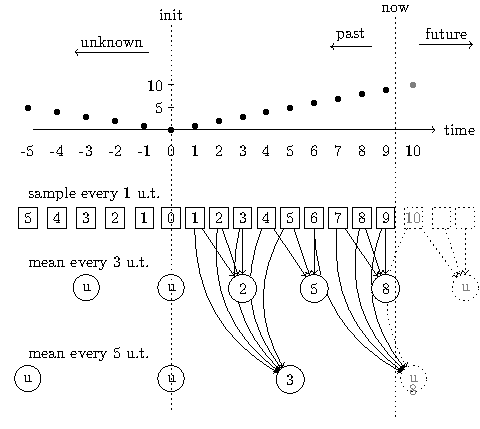
\includegraphics{fig_mtsms_sequence.pdf}
%   \caption{Multiresolution snapshot diagram with regular sampling}
%   \label{fig:mtsms:sequence}
% \end{figure}



%At the bottom of Figure~\ref{fig:mtsms:sequence} there is a diagram
showing the multiresolution action. The first row shows the numerical
time series' values corresponding to the above plot; the time series
is sampled every one unit of time. The second and the third row show a
particular schema of a multiresolution database consisting in two time
resolutions for the time series: one computes the mean of the sampled
values every three u.t.\ and the other computes the mean every five
u.t. In this example, computing the mean acts as selecting information
by aggregate statistics. All data stored before zero time is unknown
(\emph{u}) as has not been acquired. For the future values it is also
marked as \emph{u} until time advances.

The arrows of the figure show that every three sampled values a mean
is stored and, independently, every five values another mean is
stored. For the future values, dashed arrows show that if time
advances one u.t.\ then value 10 is sampled and the mean for time 10
can be computed resulting 8 but not yet the mean for time 12.









%%% Local Variables:
%%% TeX-master: "main"
%%% End:
% LocalWords: buffer buffers multiresolució SGSTM SGST





